% Source: Code/CommonSenseCarolina/latex/usc-cost-pressure.tex
% Description: Percentage increases in USC cost categories compared to cumulative CPI inflation. The dashed line marks the 31.8\% inflation baseline \citep{BLSCPI2025

\documentclass[border=4pt]{standalone}
\usepackage{graphicx}
\usepackage{pgfplots}
\usepackage{tikz}
\usepackage{xcolor}
\pgfplotsset{compat=1.18}

\definecolor{Garnet}{HTML}{73000A}
\definecolor{Atlantic}{HTML}{466A9F}
\definecolor{Congaree}{HTML}{1F414D}
\definecolor{Rose}{HTML}{CC2E40}
\definecolor{Black90}{HTML}{363636}
\definecolor{Black50}{HTML}{A2A2A2}
\definecolor{Black10}{HTML}{ECECEC}


\begin{document}
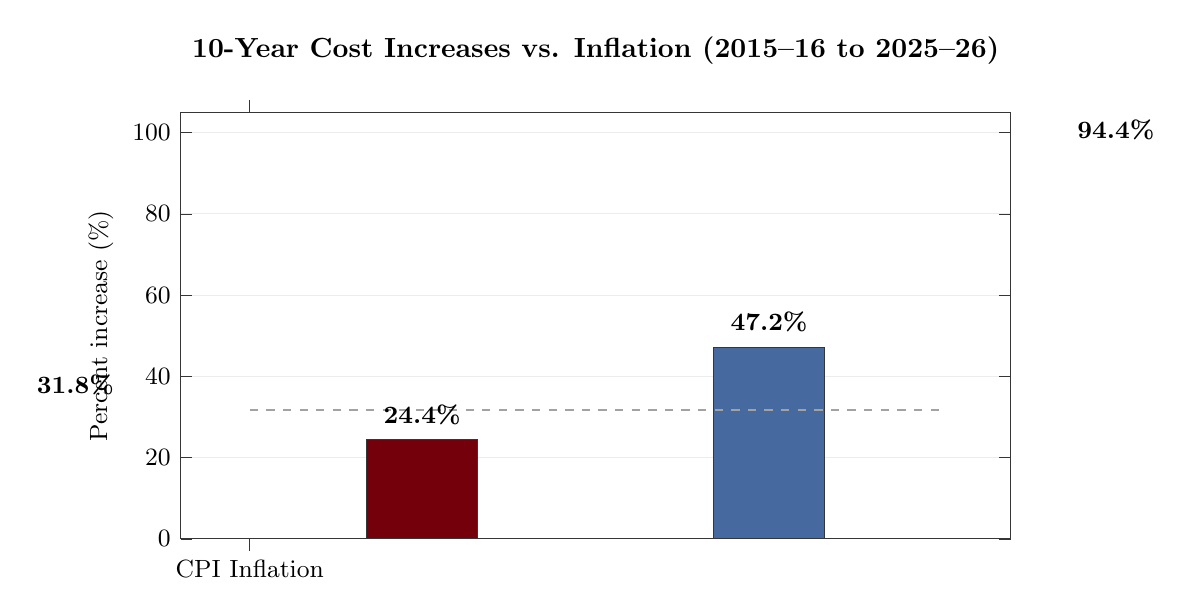
\begin{tikzpicture}
\begin{axis}[
    width=\textwidth,
    height=7cm,
    ybar,
    bar width=40pt,
    ylabel={Percent increase (\%)},
    ylabel style={font=\small},
    symbolic x coords={CPI Inflation, OOS Tuition, Housing, Meal Plan},
    xtick=data,
    xticklabel style={font=\small, rotate=0, anchor=north},
    ymin=0, ymax=105,
    ytick={0,20,40,60,80,100},
    yticklabel style={font=\small},
    ymajorgrids=true,
    grid style={color=Black10},
    axis line style={color=Black90},
    tick style={color=Black90},
    nodes near coords,
    nodes near coords style={font=\small\bfseries, anchor=south},
    every node near coord/.append style={yshift=2pt},
    point meta=explicit symbolic,
    title={\textbf{10-Year Cost Increases vs. Inflation (2015--16 to 2025--26)}},
    title style={font=\normalsize, at={(0.5,1.05)}},
]
\addplot[fill=Black50, draw=Black90] coordinates {(CPI Inflation,31.8) [31.8\%]};
\addplot[fill=Garnet, draw=Black90] coordinates {(OOS Tuition,24.4) [24.4\%]};
\addplot[fill=Atlantic, draw=Black90] coordinates {(Housing,47.2) [47.2\%]};
\addplot[fill=Rose, draw=Black90] coordinates {(Meal Plan,94.4) [94.4\%]};
\draw[dashed, thick, color=Black50] (axis cs:CPI Inflation,31.8) -- (axis cs:Meal Plan,31.8);
\end{axis}
\end{tikzpicture}
\end{document}
